
\section{Behavioral CPP Algorithm}

Following the preprocessing phase aimed at resolving the regions associated with designated points, the subsequent imperative lies in formulating an algorithm capable of comprehensively covering all identified points. With the completion of preprocessing, the focus narrows down to ensuring the precise coverage of all points to effectively identify and extract weed infestations. Although the agricultural robot in question operates under non-holonomic constraints, the overarching objective transcends mere efficiency and the identification of the shortest path. Instead, the primary emphasis lies in achieving exhaustive point coverage while strategically favoring approximately linear trajectories.

\vspace{3mm}   

The rationale behind prioritizing linear trajectories over strictly adhering to non-holonomic paths is multifaceted. Firstly, the adoption of more curved paths significantly heightens the risk of grass damage, thereby undermining the fundamental objective of preserving grass quality. Given the paramount importance of maintaining optimal grass conditions within agricultural fields, any approach that compromises this aspect inherently fails to align with the core objectives. Secondly, the energy consumption associated with traversing curved paths is substantially higher compared to linear trajectories. For the specific agricultural robot under consideration, empirical estimates suggest that traversing an equivalent path length via curved trajectories incurs an energy expenditure four times greater than that of linear paths. Consequently, the central objective of the algorithm resides in identifying the shortest path capable of encompassing all designated points while mitigating curvature and prioritizing linear trajectories.

\vspace{3mm}  

The development of this behavioral approach necessitates a nuanced understanding of agricultural terrain dynamics, robot kinematics, and energy efficiency considerations. By integrating these facets into the algorithmic design process, the resultant solution seeks to strike a delicate balance between point coverage efficacy, grass preservation, and energy optimization.


\subsection{Vision Cone Strategy: }



At this stage, having acquired comprehensive global information about the points in the field, the next step involves prioritizing straight paths while minimizing computational complexity and time. An innovative approach is employed wherein the robot is equipped with a vision cone mechanism. This vision cone is defined by two lines extending from the robot at a fixed angle and distance. The angle of these lines is determined based on the robot's minimum turning radius. For instance, for a robot with a minimum turning radius of 2 meters, the angle of the cone on either side is set at 11 degrees. The distance to the end of the cone depends on the operational area of the robot but is set to a fixed distance of 100 meters for this scenario.

\vspace{3mm}  


The vision cone allows the robot to consider only those points within this cone from its current position as potential next travel points. This selective consideration significantly reduces the computational effort required to determine the path, as it disregards points outside the cone. By narrowing the focus to relevant points within the vision cone, computational efficiency is enhanced, thus making the vision cone an intelligent and effective strategy. The vision cone can be visualized in (Figure \autoref{fig:vision_cone}).

\begin{figure}[]
    \centering
    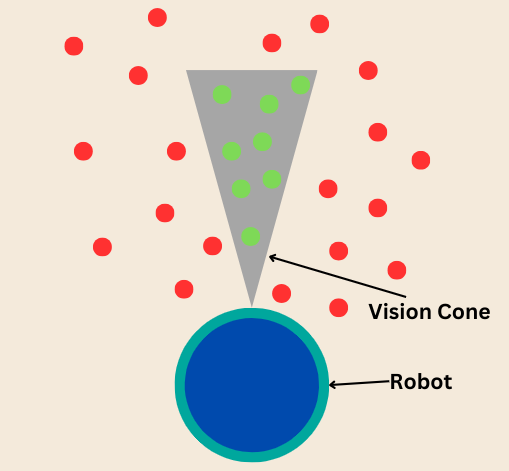
\includegraphics[width=0.3\textwidth]{Images/Algorithm_no_obs/Vision_cone.png}
    \caption{Vision Cone.}
    \label{fig:vision_cone}
\end{figure}

\subsection{Algorithmic Framework: }


The algorithmic framework is designed to facilitate comprehensive point coverage while minimizing curvature and prioritizing linear trajectories. The behavioral approach adopted for the algorithm is hierarchical, comprising three distinct behaviors that are sequentially activated. The transition from one behavior to the next is contingent upon the degree of point coverage achieved.

\begin{enumerate}
    \item \textbf{Centroid-Seeking Behavior: }The algorithm commences with the first behavior, designed to initiate coverage from the starting point. This stage focuses on covering a substantial portion of the field, leveraging the vision cone to select the next travel points and maintaining the priority on straight paths.
    
    \item \textbf{Circumferential-Traversal Behavior:} Upon achieving a certain threshold of point coverage, the algorithm transitions to the second behavior. This intermediate stage aims to further optimize coverage by adjusting the strategy based on the points that remain. The robot continues to utilize the vision cone but adopt a slightly more flexible criteria for point selection to ensure efficient coverage progression.
    
    \item \textbf{Dubins Open Travelling Salesman Problem:} Once the intermediate behavior reaches its saturation point—where additional coverage gains diminish—the algorithm shifts to the final behavior. This stage is designed to ensure complete coverage of all remaining points. The final behavior will incorporate more refined strategies to target any residual areas, ensuring no point is left uncovered.
\end{enumerate}



This hierarchical behavioral algorithm ensures a methodical and efficient approach to coverage path planning. By starting with broad coverage strategies and progressively refining the approach, the algorithm effectively balances the need for comprehensive point coverage with the constraints of the robot's kinematic capabilities and the operational goal of preserving grass quality. The pseudocode for the complete coverage path planning algorithm is provided in (Algorithm \autoref{alg:completebehavioralalgorithm}). 

\vspace{3mm}   

Convention to be followed for the algorithms:
\begin{multicols}{2}
\begin{itemize}[noitemsep,topsep=0pt]
    \item $P$: path.
    \item $p$: points.
    \item $r$: robot.
    \item $R$: Radius.
    \item $VC$: Vision cone.
    \item $C$: Centroid.
    \item $N_s$: Number of sample orientations.
    \item $ \delta$: Percentage.
    \item $step$: Step size.
    \item $O$: Orientation.
\end{itemize}
\end{multicols}

\vspace{3mm}  

Notations for CompleteBehavioralAlgorithm:
\begin{multicols}{2}
\begin{itemize}[noitemsep,topsep=0pt]
    \item $p_{cl}$: clustered points.
    \item $p_r$: remaining points.
    \item $\delta_{\text{bc}}$: behavior change percentage.
    \item $\delta_c$: coverage percentage.
    \item $P_c$: completed path.
    \item $P_s$: straight path.
    \item $R_{\text{conc}}$: concurrent region radii.
    \item $P_d$: Dubins path.
    \item $P_{dotsp}$: DOTSP path.
    \item $P_{cd}$: Complete Dubins path.
\end{itemize}
\end{multicols}

\begin{algorithm}[H]
    \caption{CompleteBehavioralAlgorithm}
    \label{alg:completebehavioralalgorithm}
    \begin{algorithmic}[1]
    \Statex \textbf{Input:} 2D points ($p_{2d}$), initial robot pose ($r_{\text{pos}}$), turning radius ($R_{\text{tu}}$) 
    \Statex \textbf{Output:} Dubins path $P_{cd}$
    \newline

    \State $p_{cl}, \delta_{\text{bc}} \leftarrow$ CentroidsAndAutoBehaviorShift($P_{2d}$, $R_{\text{min}}$, $R_{\text{max}}$, $N$ )
    \State $p_r \leftarrow p_{cl}$
    \State $\delta_c \leftarrow 0$
    \State $P_c \leftarrow []$
    
    \While{True}
        \If{$\delta_c <  \delta_{\text{bc}}$}
            \State $P_s, p_r \leftarrow$ Behavior\_1($p_r$, $p_{cl}$, $N_s$, $r_{\text{pos}}$, $VC$, $C$, $R_{\text{conc}}$, $step$)
        \Else
            \State $P_s, p_r \leftarrow$ Behavior\_2($p_r$, $p_{cl}$, $N_s$, $r_{\text{pos}}$, $VC$, $C$, $R_{\text{conc}}$, $step$)
        \EndIf
        
        \State $P_c \mathrel{+}= P_s$
        \State $r_{\text{pos}} \leftarrow P_c[-1]$
        \State $\delta_c \leftarrow$ UpdateCoveragePerc($P_c$, $p_r$)
        
        \If{$\text{len}(P_s) == 0$}
            \State \textbf{break}
        \EndIf
    \EndWhile
    
    \State $P_d \leftarrow$ DubinsPath($P_c$, $R_{\text{tu}}$)
    \State $P_{dotsp} \leftarrow$ DOTSPPath($p_r$, $r_{pos}$, $R_{\text{tu}}$)
    \State $P_{cd} \leftarrow P_d + P_{dotsp}$

    \State \Return $P_{cd}$
    \end{algorithmic}
\end{algorithm}
    

\subsection{Rationale for Hierarchical Approach: } 


The hierarchical approach is adopted to improve convergence rate and coverage efficiency. If a single algorithm or behavior were followed throughout, the robot would cover many points initially but gradually cover fewer points over time, reducing the algorithm's accuracy and increasing the overall path length and operational time. By transitioning between different behaviors, the algorithm can adapt to the changing density and distribution of points, maintaining high efficiency throughout the coverage process.

\vspace{3mm}   


This hierarchical strategy ensures that the algorithm remains effective even as the number of uncovered points decreases. By tailoring the approach to the specific conditions encountered at each stage, the robot can optimize its path, reduce unnecessary movements, and maintain high precision in point coverage. This not only conserves energy but also preserves the quality of the grass by minimizing excessive traversal. The adaptive nature of the hierarchical approach thus represents a robust and efficient solution for coverage path planning in agricultural fields. 





\subsection{Centroid-Seeking Behavior}


The algorithm begins by receiving the centroids of the overlaps between the regions of the raw points as input. It takes the initial position and orientation of the robot, where the position remains fixed while the orientation is treated as a temporary orientation. From this temporary orientation, the algorithm considers an angular range of twenty-four degrees on either side. Within this range, it samples six orientations on each side, resulting in a total of thirteen orientations, including the initial orientation. 

\vspace{3mm}   

The algorithm designates the current orientation as the leftmost extreme orientation. Using this position and orientation, it then starts selecting the next point to navigate to. At this stage, the algorithm employs the vision cone mechanism, characterized by an 11-degree angle on either side and extending 100 meters forward. The primary objective at this juncture is to select the next most suitable point within the vision cone.

\vspace{3mm}  

To determine the next best suitable point, the algorithm extracts the five closest points from the current position and orientation within the vision cone. These points are regarded as semi-potential points. For each of these semi-potential points, the algorithm computes the distribution of points on either side of the current orientation across the entire vision cone. A combined score is then calculated for each semi-potential point based on the distance from the robot and the total distribution of points in the vision cone. Both the distance and the distribution are normalized before calculating the combined score. The semi-potential point with the highest combined score is deemed the best potential candidate and is selected as the next point to navigate to. This scoring method is intelligent as it considers not only the distance but also the future distribution of points, thereby facilitating more efficient coverage as the robot progresses.

\vspace{3mm}  

Once the best potential point is selected, it becomes the next point for navigation. The robot's orientation at this new point is updated based on the direction vector from the robot to the selected point. The robot then moves to this potential point with the updated orientation. This process is repeated, with the robot continually navigating to the next potential point until no points are visible within the vision cone. This pattern encourages the robot to move in an approximately straight line whenever possible. When the robot can no longer find any points within the vision cone, it indicates that the robot has reached the extreme end of the points and is considered as one temporary turn. At this point, the number of points covered in this orientation is recorded.

\vspace{3mm}  

\textbf{Returning to Initial Position and Orientation}

After completing one temporary turn, the robot will return to its starting position and orientation. The robot then considers the next orientation in the set of thirteen sampled orientations and proceeds to complete an approximately straight path in that direction, recording the number of points covered along each path. This process is repeated for all thirteen orientations. Upon completing paths for all orientations, the orientation that results in the maximum number of points covered is selected as the optimal orientation for further navigation.
\vspace{3mm}  

\textbf{Incorporating Non-Holonomic Constraints for Turns}

When making a turn, the robot must adhere to its non-holonomic constraints. To address this, the algorithm considers a circular region around the robot with defined minimum and maximum radii. The minimum radius is set to one and a half times the robot's minimum turning radius, ensuring feasible turns. The initial maximum radius is set to three times the minimum turning radius. If no points are found within this initial circular region, the outer radius is incrementally increased by two units until the maximum radius limit is reached.
\vspace{3mm}  

Within this circular region, the algorithm identifies all potential points and filters them further. The selection process involves evaluating each point based on a combined score, considering both the distance from the robot and the angle differnce between the robot's orientation and the vector from the robot to the potential point. both the entities are normalized before comparison. A lower distance and a smaller orientation deviation result in a higher score for the point. The point with the highest score is selected as the next potential point for the robot to navigate to when making a turn.
\vspace{3mm}  

\textbf{Orientation Towards Centroid}

At the beginning of the algorithm, the centroid of the entire set of points is computed. When selecting a point for the turn, the orientation is determined by the vector from the selected point towards this centroid. This selected point becomes the next navigation target, and the orientation towards the centroid becomes the new temporary orientation for the robot.

\vspace{3mm}  

\textbf{Continuing the Path and Making Turns}

Upon reaching the end of a complete path, the robot needs to execute a turn. This turn is represented by a single completed path, after which the robot continues the same pattern of operation. From the point where the turn is made, the robot selects thirteen orientations and navigates along each one, completing a path and recording the number of points covered. The orientation that results in the maximum number of points covered is then selected as the optimal orientation for continued navigation. This process is iterative and continues throughout the first behavior.

\vspace{3mm}  

\textbf{Focus on Points Near the Centroid:}

This first behavior of the robot emphasizes covering more points near the centroid of the data and not covering points on the outer sides. Initially, the robot covers a significant number of points with each path. However, as the number of turns increases, the coverage rate decreases. This reduction in efficiency occurs because the robot focuses on points near the centroid as after each turn it faces toward the centroid, resulting in majority of the points covered are in the central region. Consequently, while this behavior ensures substantial coverage, it becomes less efficient over time as fewer new points are covered with each turn.

\vspace{3mm}  


The first behavior algorithm can be visualized in (Algorithm \autoref{alg:behavioral1})

\vspace{3mm}  

Notations for Behavior 1 and 2:
\begin{multicols}{2}
    \begin{itemize}[noitemsep,topsep=0pt]
        \item $P_{cs}$: Complete straight path
        \item $P_{t}$: Temporary path
        \item $p_{co}$: Points covered
        \item $O_{sa}$: Sampled orientations
        \item $p_v$: Visible points
        \item $p_{po}$: Potential point
        \item $O_n$: New orientation
        \item $p_{int}$: Intermediate points
        \item $O_{bi}$: Best orientation index
        \item $P_{tu}$: Turn point
        \item $O_b$: Best orientation
    \end{itemize}
\end{multicols}

\begin{algorithm}[H]
    \caption{Behavior\_1}
    \label{alg:behavioral1}
    \begin{algorithmic}[1]

    \Statex \textbf{Input:} 2D points ($P_{2d}$), clustered points ($p_{cl}$), number of sample orientations ($N_s$), robot pose ($r_{pos}$), vision cone ($VC$), centroid ($C$), concurrent region radii ($R_{\text{conc}}$), step size ($S$)

    \Statex \textbf{Output:} Complete straight path $P_{cs}$, remaining points $p_r$
    \newline
    \State $P_{cs} \leftarrow []$
    \State $P_t \leftarrow [[] \text{ for } \_ \text{ in range}(N_s)]$
    \State $p_{co} \leftarrow [[] \text{ for } \_ \text{ in range}(N_s)]$
    \State $O_{sa} \leftarrow$ SampleTheOrientations($R_{pos}[2]$, $N_s$, $S$)
    
    \For{$i, O$ \textbf{in} $O_{sa}$}
        \State $R_{pos}[2] \leftarrow O$
        \While{no point is visible}
            \State $p_v \leftarrow$ ComputeVisionConePoints($r_{pos}$, $VC$)
            \State $p_{po} \leftarrow$ FindPotentialPoint($r_{pos}$, $p_v$)
            \If{$p_{po}$ is None}
                \State \textbf{break}
            \EndIf
            \State $O_n \leftarrow$ FromCurrentPoseToPotentialPoint($r_{pos}$, $p_{po}$)
            \State $P_t[i].\text{append}([p_{po}, O_n])$
            
            \State $p_{int} \leftarrow$ CheckIntermediatePoints($p_r$)
            \State $P_t[i].\text{append}(p_{int})$
            \State $p_c[i].\text{append}(\text{len}(P_t))$
            \State $p_r \leftarrow p_{cl} - P_t$
            \State $r_{pos} \leftarrow [p_{po}, O_n]$
        \EndWhile
    \EndFor
    
    \State $O_{bi} \leftarrow \text{argmax}(p_c[:])$
    \State $P_{cs} \leftarrow P_t[O_{bi}]$
    
    \State $r_{pos} \leftarrow P_{cs}[-1]$
    \State $p_{tu} \leftarrow$ PotentialPointToTurn($p_r$, $R_{\text{conc}}$, $r_{pos}$)
    \State $O_b \leftarrow$ TowardsCentroid($p_{tu}$, $C$)
    \State $P_{cs}.\text{append}([p_{tu}, O_b])$
    \State $p_r.\text{remove}([p_{tu}])$
    
    \State \Return $P_{cs}$, $p_r$
    \end{algorithmic}
    \end{algorithm}
    


\subsection{Circumferential-Traversal Behavior:} 

Circumferential-Traversal Behavior is designed to enhance the coverage rate and improve the convergence efficiency. Upon transitioning from the first to the second behavior, the algorithm takes all remaining points as input, considering the current position and orientation of the robot. At this stage, the density of uncovered points is lower near the centroid and higher towards the boundaries of the operational area. Therefore, the second algorithm focuses on covering points located along the periphery rather than near the centroid.

\vspace{3mm}   

\textbf{Orientation Sampling and Path Selection:}

The algorithm begins similarly by selecting thirteen orientations from the robot's current position and orientation. The robot navigates along each orientation, completing a path and recording the number of points covered. The orientation resulting in the highest number of points covered is selected as the optimal direction for continued navigation. This ensures that the robot always moves in the direction that maximizes point coverage.

\vspace{3mm}   

\textbf{Refined Criteria for Selecting Turning Points:}

A critical difference in the second behavior lies in the method for selecting the orientation of the next best point to make a turn. The algorithm considers a circular region around the robot with predefined minimum and maximum radii similarly as of first behavior and computes the potential points based on distance and orientation difference. By doing so, the algorithm ensures that the robot makes smooth, efficient turns that align with its non-holonomic constraints.

\vspace{3mm}   

The point with the least orientation difference and the shortest distance is chosen as the next point for making a turn. Unlike the first behavior, where the orientation towards the centroid was prioritized, the orientation of this potential point is directed towards the next point along the same moving orientation. For example, if the potential point lies clockwise to the robot's current orientation, the robot's new orientation will aim towards the next nearest point with the smallest clockwise orientation difference, and the same applies for counterclockwise points. This new orientation becomes the temporary orientation, and the robot continues the process of orientation sampling and selection with the goal of maximizing point coverage.

\vspace{3mm}   

Enhanced Coverage and Convergence: This behavior is particularly effective in covering points along the boundaries and in regions with higher point density, thereby increasing the overall coverage rate and convergence efficiency of the algorithm. While the first behavior predominantly focuses on points near the centroid, the second behavior shifts attention to the boundary points, ensuring a more balanced and comprehensive coverage pattern.


\vspace{3mm}   

Enhancing Coverage with Intermediate Points: To further improve the coverage rate and convergence of the algorithm, an additional mechanism is incorporated into both the first and the second behaviors. This enhancement involves covering intermediate points along each path between two selected points. The algorithm checks for points that lie close to the current path within a certain threshold distance.

\vspace{3mm}   

The orientation for these intermediate points is determined based on their position. If multiple points exist close to the path, the orientation is directed towards the next intermediate point in sequence. For the last intermediate point, the orientation is towards the final end point.

\vspace{3mm}   

Another criterion for selecting intermediate points depends on the distance between the end points of the path. If this distance is substantial, points that are slightly farther but within the threshold are also considered. In such cases, the algorithm allows for a minor compromise on the straightness of the path to cover more points, thereby further enhancing the coverage rate and convergence efficiency.

\vspace{3mm}   

Efficiency of Combined Behaviors: Both the first and second behaviors, along with the enhancement for intermediate points, ensure complete coverage of the points. These behaviors have been experimentally validated to provide good coverage rates and convergence for the algorithm. However, the efficiency in terms of coverage rate, convergence speed, and path length diminishes after approximately eighty-five to ninety percent of the points are covered. At this stage, the algorithm tends to cover fewer points per turn and makes multiple turns to cover just two or three points.

\vspace{3mm}   

This inefficiency results in longer paths and higher energy consumption, which contradicts the goal of minimizing path length and conserving energy. This challenge highlights the necessity for a third behavior. The third behavior aims to optimize the coverage of remaining points by allowing slight deviations from straight paths to cover more points efficiently, thus reducing the overall path length and energy consumption.

\vspace{3mm}   

The pseudocode for the second behavior algorithm is shown in (Algorithm \autoref{alg:behavioral2})

\begin{algorithm}[H]
    \caption{Behavior\_2}
    \label{alg:behavioral2}
    \begin{algorithmic}[1]

    \Statex \textbf{Input:} 2D points ($P_{2d}$), clustered points ($p_{cl}$), number of sample orientations ($N_s$), robot pose ($r_{pos}$), vision cone ($VC$), centroid ($C$), concurrent region radii ($R_{\text{conc}}$), step size ($S$)

    \Statex \textbf{Output:} Complete straight path $P_{cs}$, remaining points $p_r$
    \newline
    \State $P_{cs} \leftarrow []$
    \State $P_t \leftarrow [[] \text{ for } \_ \text{ in range}(N_s)]$
    \State $p_{co} \leftarrow [[] \text{ for } \_ \text{ in range}(N_s)]$
    \State $O_{sa} \leftarrow$ SampleTheOrientations($R_{pos}[2]$, $N_s$, $S$)
    
    \For{$i, O$ \textbf{in} $O_{sa}$}
        \State $R_{pos}[2] \leftarrow O$
        \While{no point is visible}
            \State $p_v \leftarrow$ ComputeVisionConePoints($r_{pos}$, $VC$)
            \State $p_{po} \leftarrow$ FindPotentialPoint($r_{pos}$, $p_v$)
            \If{$p_{po}$ is None}
                \State \textbf{break}
            \EndIf
            \State $O_n \leftarrow$ FromCurrentPoseToPotentialPoint($r_{pos}$, $p_{po}$)
            \State $P_t[i].\text{append}([p_{po}, O_n])$
            
            \State $p_{int} \leftarrow$ CheckIntermediatePoints($p_r$)
            \State $P_t[i].\text{append}(p_{int})$
            \State $p_c[i].\text{append}(\text{len}(P_t))$
            \State $p_r \leftarrow p_{cl} - P_t$
            \State $r_{pos} \leftarrow [p_{po}, O_n]$
        \EndWhile
    \EndFor
    
    \State $O_{bi} \leftarrow \text{argmax}(p_c[:])$
    \State $P_{cs} \leftarrow P_t[O_{bi}]$
    
    \State $r_{pos} \leftarrow P_{cs}[-1]$
    \State $p_{tu} \leftarrow$ PotentialPointToTurnCCW($p_r$, $R_{\text{conc}}$, $r_{pos}$)
    \State $O_b \leftarrow$ VectorsTowardsNextCCWPoint($p_{tu}$, $p_r$)
    \State $P_{cs}.\text{append}([p_{tu}, O_b])$
    \State $p_r.\text{remove}([p_{tu}])$

    \State \Return $P_{cs}$, $p_r$
    \end{algorithmic}
    \end{algorithm}
    


\subsection{Dubins open travelling salesman problem (DOTSP):}



The final behavior addresses the coverage of the remaining points, which are sparsely distributed across the area. At this stage, the concept of the vision cone is removed, as maintaining strict straightness is no longer prioritized. Although straight paths are typically more energy-efficient, the robot would consume more energy traveling long straight paths while covering fewer points. Instead, small circular turns with a radius of 3 meters are preferred, allowing the robot to avoid long straight paths of up to 100 meters. This approach optimizes energy usage by prioritizing the coverage of remaining points over path straightness.

\vspace{3mm}   

To determine the optimal path for these remaining points, the algorithm employs the Dubins open traveling salesman problem (TSP). DOTSP extends the open TSP by accounting for the non-holonomic constraints of vehicles, such as turning radius and orientation. It seeks to find the shortest path that visits a set of points while respecting the vehicle's kinematic constraints. 

\vspace{3mm}   

Initially, the shortest path between the points is computed using the open TSP. Subsequently, Dubins constraints are applied to ensure the path is feasible for the robot. This method not only ensures complete coverage of the remaining points but also reduces the overall path length and energy consumption. By adopting this approach, the algorithm significantly improves the coverage rate and convergence speed, achieving comprehensive coverage in an efficient manner. The pseudocode for the DOTSP behavior algorithm is shown in (Algorithm \autoref{alg:dotsp_path}). An example of the DOTSP path is shown in \autoref{fig:dotsp_path}.

% selected field region. 
\begin{figure}[H]
    \centering
    \begin{tabular}{cc} 
        \begin{subfigure}{0.5\textwidth}
            \centering
            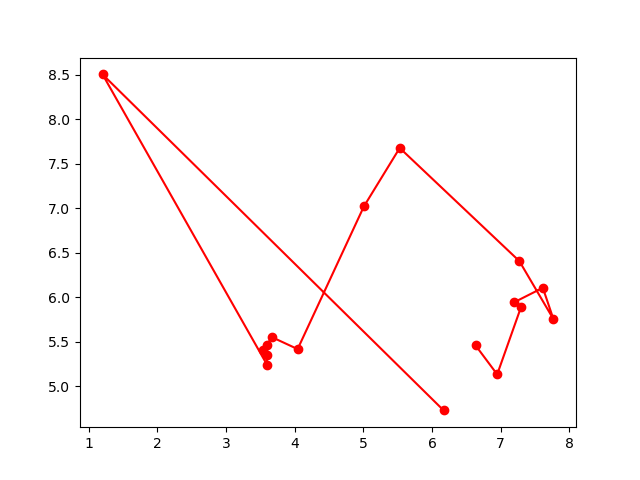
\includegraphics[width=\textwidth]{Images/Algorithm_no_obs/OTSP.png}
            \caption{TSP path for remaining points.}
        \end{subfigure} 
        &
        \begin{subfigure}{0.5\textwidth}
            \centering
            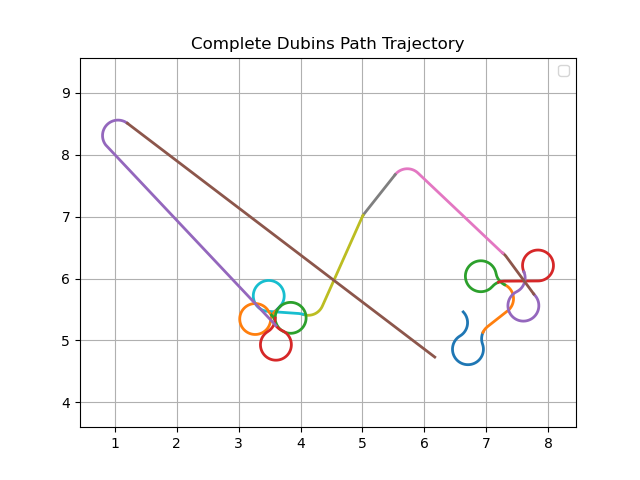
\includegraphics[width=\textwidth]{Images/Algorithm_no_obs/tsp_dubins_path.png}
            \caption{DOTSP path for remaining points.}
        \end{subfigure}
    \end{tabular}
    \caption{Centroids of overlapped regions.\label{fig:dotsp_path}} 
\end{figure}

Notations for DOTSP:
\begin{multicols}{2}
\begin{itemize}[noitemsep,topsep=0pt]
    \item $sn$: Start node
    \item $G$: Graph
    \item $P_{clo}$: Closed path
    \item $P_{op}$: Open path
    \item $P_{dotsp}$: DOTSP path
\end{itemize}
\end{multicols}

\begin{algorithm}[H]
    \caption{DOTSP}
    \label{alg:dotsp_path}
    \begin{algorithmic}[1]
    \Statex \textbf{Input:} remaining points ($p_r$), initial robot position( $r_{\text{pos}}$), turning radius ($R_{\text{tu}})$
    \Statex \textbf{Output:} Dubins path ($P_{dotsp}$)
    \newline
    \State $sn \leftarrow r_{\text{pos}}$
    \State $G \leftarrow$ GenerateGraph($p_r$)
    \State $P_{clo} \leftarrow$ SolveClosedTSP($G$, $sn$)
    \State $P_{op} \leftarrow$ RemoveEdgeWithMaxWeightFromStartNode($G$, $sn$)
    \State $P_{dotsp} \leftarrow$ DubinsPath($P_{op}$, $R_{\text{tu}}$)
    \State \Return $P_{dotsp}$
    \end{algorithmic}
    \end{algorithm}

This integrated strategy, comprising the first, second, and final behaviors, enables the robot to cover all points in the agricultural field effectively. Each behavior is tailored to optimize different stages of the coverage process, from focusing on dense central areas to sparsely populated boundaries and finally to the remaining isolated points. This hierarchical and adaptive approach ensures that the robot operates efficiently, minimizing both path length and energy consumption throughout the coverage process.



\subsection{Automatic Shift Between Behaviors: }
A critical aspect of this behavioral algorithm is the decision-making process for shifting from one behavior to the next. Different data distributions require varying coverage percentages to optimize this transition. Determining the optimal shift point is challenging and necessitates extensive experimentation and testing to achieve the best coverage rate and convergence.

\vspace{3mm}   

The performance of the algorithm can significantly vary depending on when the shift between behaviors occurs. For the same dataset, different coverage percentages for behavior shifts can greatly influence the coverage rate and convergence efficiency. Therefore, it is essential to tailor the shift points for each specific dataset rather than relying on a fixed percentage.

\vspace{3mm}   

One of the standout features of this behavioral algorithm is its ability to determine the near-optimal coverage percentage for shifting behaviors. Once the dataset is pre-processed, the algorithm computes the best percentage coverage for behavior shifts as follows:

\begin{itemize}
    \item \textbf{Centroid and Concentric Circles:  }The algorithm first computes the centroid of the dataset. Imaginary concentric circles are then centered at the centroid, with varying radii extending outward until all points are encompassed.
    \item \textbf{Point Distribution Analysis:  }The percentage of points within each concentric region is calculated. The behavioral shift percentage is determined based on a threshold percentage found through experimentation and testing, which is 50 percent. The points are counted in each region, starting from the innermost circle, and the percentages are accumulated until the threshold is reached.
    \item \textbf{Threshold Determination:  }The region where the threshold percentage is exceeded dictates the coverage percentage for the behavior shift. If the threshold is reached in the innermost region, indicating a dense point distribution near the centroid, the first behavior will be more effective, and the shift percentage will be automatically set to a higher percent (e.g., 60-70\%). Conversely, if the threshold is reached in the outer regions, suggesting denser distribution near the boundaries, the second behavior becomes more pertinent, and the shift percentage is automatically set to a lower percent (e.g., 30-40\%) by the algorithm. 
\end{itemize} 

This intellectually behavior shifting enables the algorithm to determine the optimal coverage percentage, thereby enhancing the overall coverage rate and convergence efficiency. By integrating these calculated shift points, the hierarchical behavioral algorithm adapts dynamically to different datasets, ensuring that the robot operates efficiently across various scenarios. The pseudocode for the Auto-Shift behavior algorithm is shown in (Algorithm \autoref{alg:autobehaviorshift}). The concept of concentric circles, centroids and the points distribution considered for the automatic shift between behaviors can be visualized in the (\autoref{fig:auto_shift}).


\begin{figure}[H]
    \centering
    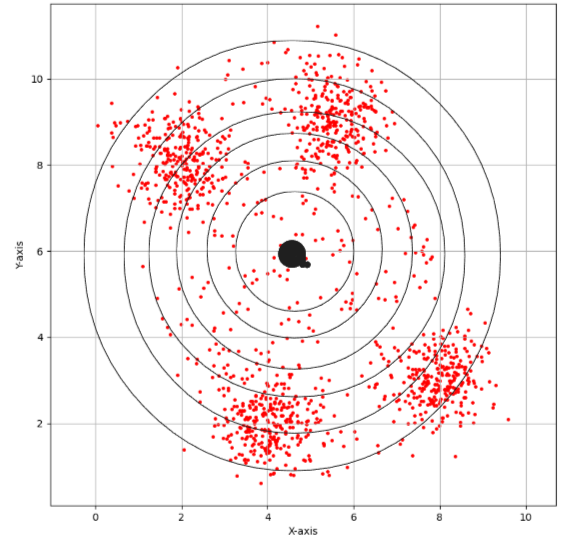
\includegraphics[width=0.5\textwidth]{Images/Algorithm_no_obs/auto.png}
    \caption{CCP Behavioral Algorithm flowchart.}
    \label{fig:auto_shift}
\end{figure}


Notations for AutoBehaviorShift:
\begin{multicols}{2}
    \begin{itemize}[noitemsep,topsep=0pt]
        \item $\delta_to$: Total percentage
        \item $\delta_{th}$: Threshold percentage
        \item $\delta_{list}$: List of percentages
        \item $cc$: Concentric circles
        \item $R_{cu}$: Current radius
        \item $p_{cu_\delta}$: Percentage of points in subregion
    \end{itemize}
\end{multicols}

\begin{algorithm}[H]
    \caption{AutoBehaviorShift}
    \label{alg:autobehaviorshift}
    \begin{algorithmic}[1]
    \Statex \textbf{Input: }  \textit{2D points} ($P_{2d}$), \textit{min\_radius} ($R_{\text{min}}$),  \textit{max\_radius} ($R_{\text{max}}$), number of concurrent circles ($N$) 
    \Statex \textbf{Output: } \textit{behavior\_change\_percent} $\delta_{\text{bc}}$ 
    \newline
    \State $\delta_{to} \leftarrow 0$ 
    \State $\delta_{th} \leftarrow 50$ 
    \State $\delta_{list} \leftarrow \text{GeneratePercentageList}(30, 80, N)$ \Comment{List from 30 to 80\% with N steps.}
    \State $cc \leftarrow \text{ConcentricCircles}(P_{2d}$, $R_{\text{min}}$, $R_{\text{max}}$, $N$)
    \For{$i, R_{cu}$ \textbf{in} $cc$}
        \State $p_{cu_\delta} \leftarrow \text{PointsPercentageInSubregion}(R_{cu})$
        \State $\delta_{to} \leftarrow \delta_{to} + p_{cu_\delta}$
        \If{$\delta_{to} > \delta_{th}$}
            \State $\delta_{\text{bc}} \leftarrow \delta_{list}[i]$
            \State \textbf{break}
        \EndIf
    \EndFor
    \State \Return $\delta_{\text{bc}}$
    \end{algorithmic}
    \end{algorithm}


The flowchart of the complete behavioal algorithm can be visualized in the (\autoref{fig:ccp_flowchart_no_obs})


% Include an image
\begin{figure}[H]
    \centering
    \includegraphics[height=22cm, width=\textwidth]{Images/flowchart/flowchart_no_obs_new.pdf}
    \caption{CCP Behavioral Algorithm flowchart.}
    \label{fig:ccp_flowchart_no_obs}
\end{figure}